% Fig. 3 -- Threat model: adversary capability, entry point, countermeasure (single column, 3.5 in).
% Compile with pdfLaTeX (Overleaf default). Output: fig03_threat_model.pdf
\documentclass[border=3pt]{standalone}
\usepackage[T1]{fontenc}
\usepackage{newtxtext,newtxmath}
\usepackage{tikz}
\usetikzlibrary{arrows.meta,positioning,calc}

\definecolor{acc}{RGB}{31,78,121}
\colorlet{accfill}{acc!10}
\colorlet{gfill}{black!7}

\tikzset{
  >={Stealth[length=3pt,width=2.6pt]},
  every node/.style={font=\footnotesize},
  col1/.style={draw=black,line width=0.5pt,fill=gfill,align=left,inner sep=2.5pt,
               text width=68pt,minimum height=34pt},
  col2/.style={draw=black,line width=0.5pt,fill=white,align=left,inner sep=2.5pt,
               text width=56pt,minimum height=34pt},
  col3/.style={draw=acc,line width=0.7pt,fill=accfill,align=left,inner sep=2.5pt,
               text width=76pt,minimum height=34pt},
  head/.style={align=center,font=\footnotesize\bfseries},
  flow/.style={->,line width=0.5pt},
}

\begin{document}
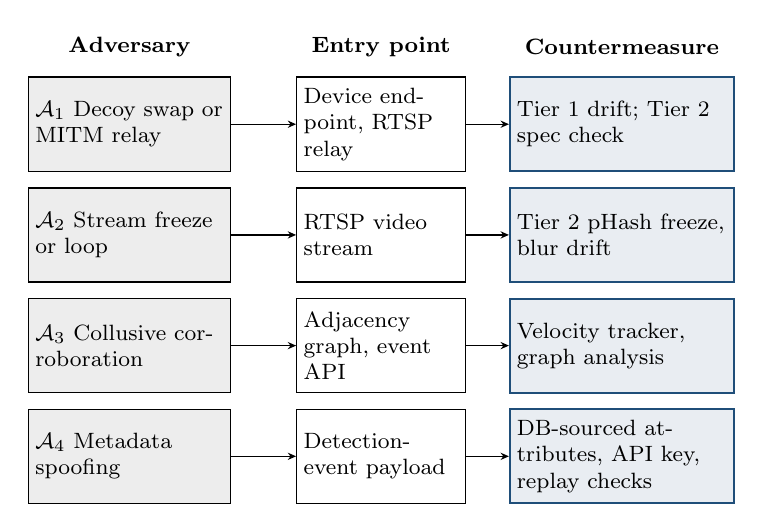
\begin{tikzpicture}[x=1pt,y=1pt]
  % headers (column centres: 36, 127, 214)
  \node[head] at (36,0)  {Adversary};
  \node[head] at (127,0) {Entry point};
  \node[head] at (214,0) {Countermeasure};

  % rows
  \node[col1] (r1a) at (36,-28)  {$\mathcal{A}_1$ Decoy swap or MITM relay};
  \node[col2] (r1b) at (127,-28) {Device endpoint, RTSP relay};
  \node[col3] (r1c) at (214,-28) {Tier 1 drift; Tier 2 spec check};

  \node[col1] (r2a) at (36,-68)  {$\mathcal{A}_2$ Stream freeze or loop};
  \node[col2] (r2b) at (127,-68) {RTSP video stream};
  \node[col3] (r2c) at (214,-68) {Tier 2 pHash freeze, blur drift};

  \node[col1] (r3a) at (36,-108)  {$\mathcal{A}_3$ Collusive corroboration};
  \node[col2] (r3b) at (127,-108) {Adjacency graph, event API};
  \node[col3] (r3c) at (214,-108) {Velocity tracker, graph analysis};

  \node[col1] (r4a) at (36,-148)  {$\mathcal{A}_4$ Metadata spoofing};
  \node[col2] (r4b) at (127,-148) {Detection-event payload};
  \node[col3] (r4c) at (214,-148) {DB-sourced attributes, API key, replay checks};

  \foreach \i in {1,2,3,4}{
    \draw[flow] (r\i a.east) -- (r\i b.west);
    \draw[flow] (r\i b.east) -- (r\i c.west);
  }
\end{tikzpicture}
\end{document}
